% vim: spelllang=en_gb

\documentclass[12pt,a4paper,draft]{scrartcl}
\usepackage{ifdraft}

% --------------------
% Set Language Options
% --------------------

\usepackage[nswissgerman,french,main=english]{babel}
\usepackage[autostyle,english=american,german=swiss]{csquotes}
\MakeOuterQuote{"}

\usepackage[shortcuts]{extdash}

% --------------
% Font & Symbols
% --------------

\usepackage{amssymb,mathtools}
\usepackage[warnings-off={mathtools-colon,mathtools-overbracket}]{unicode-math}
\usepackage[oldstyle,proportional]{libertinus-otf}

% ---------------
% Set Page Layout
% ---------------

% Get length of 65 characters
%\setlxvchars

\usepackage[driver=auto]{geometry}
% A5: 148mm × 210mm
% A4: 210mm × 297mm
\geometry{
  width=140mm,
  height=217mm,
  marginparsep=3mm,
  marginparwidth=30mm,
}
\ifdraft{\geometry{
  inner=10mm,
  marginparwidth=50mm
}}{}


% ---------------------
% Load Various Packages
% ---------------------

% Various Math Environments
\usepackage{amsthm,thmtools}
\usepackage{physics} % various shortcuts

% Bibliography
\usepackage{biblatex}
\addbibresource{bibliography.bib}

% For general figures
\usepackage[final]{graphicx}
\graphicspath{{/img}}
\usepackage{subcaption}
\usepackage{tikz}
\usetikzlibrary{babel,cd,shapes,3d}
\tikzcdset{arrow style=math font}
\tikzset{cross/.style={
    cross out, draw, solid, thin, 
    minimum size=2*(#1-\pgflinewidth), 
    inner sep=0pt, outer sep=0pt
  },
  cross/.default={3},
  conic/.pic={
    \begin{scope}[canvas is xz plane at y=0]
      \draw (0,0) circle [radius=0.5];
    \end{scope}
    \begin{scope}[canvas is xz plane at y=1]
      \draw (0,0) circle [radius=0.8];
    \end{scope}
    \begin{scope}[canvas is xz plane at y=-1]
      \draw (-20:.8) arc [start angle=-20,end angle=160,radius=.8];
      \draw[dotted] (160:.8) arc [start angle=160,end angle=340,radius=.8];
    \end{scope}
    \begin{scope}[rotate around y=20]
      \draw (.8,1) .. controls +(0,0) and +(0,.3) .. (0.5,0) .. controls +(0,-0.3) and +(0,0) .. (.8,-1);
      \draw (-.8,1) .. controls +(0,0) and +(0,.3) .. (-0.5,0) .. controls +(0,-0.3) and +(0,0) .. (-.8,-1);
    \end{scope}
  },
  degenerate conic/.pic={
    \begin{scope}[canvas is xz plane at y=1]
      \draw (0,0) circle [radius=.8];
    \end{scope}
    \begin{scope}[canvas is xz plane at y=-1]
      \draw (-20:.8) arc [start angle=-20,end angle=160,radius=.8];
      \draw[dotted] (160:.8) arc [start angle=160,end angle=340,radius=.8];
    \end{scope}
    \begin{scope}[rotate around y=20]
      \draw (-.8,-1) -- (.8,1);
      \draw (-.8,1) -- (.8,-1);
    \end{scope}
  },
  reduced conic/.pic={
    \begin{scope}[canvas is xz plane at y=1]
      \draw[very thin, opacity=0.5] (0,0) circle [radius=.8];
      \draw (-32:.8) arc [start angle=-32,end angle=32,radius=.8];
    \end{scope}
    \begin{scope}[canvas is xz plane at y=-1]
      \draw[very thin, opacity=0.5] (0,0) circle [radius=.8];
      \draw (-32:.8) arc [start angle=-32,end angle=32,radius=.8];
    \end{scope}
    \begin{scope}[canvas is xz plane at y=0]
      \draw[very thin, opacity=0.5] (0,0) circle [radius=.5];
      \draw (-32:.5) arc [start angle=-32,end angle=32,radius=.5];
    \end{scope}
    \foreach \φ in {32,-32} {
      \begin{scope}[rotate around y=\φ]
        \draw (.8,1) .. controls +(0,0) and +(0,.3) .. (0.5,0) .. controls +(0,-0.3) and +(0,0) .. (.8,-1);
      \end{scope}
    }
    \begin{scope}[rotate around y=20]
      \draw[very thin, opacity=0.5] (-.8,1) .. controls +(0,0) and +(0,.3) .. (-0.5,0) .. controls +(0,-0.3) and +(0,0) .. (-.8,-1);
    \end{scope}
  }
}

% For lists
\usepackage[shortlabels]{enumitem}

% For better Tables
\usepackage{tabularray}

% For more fine grained typesetting in final mode.
% Else set the tolerance for overfull warnings higher.
\ifdraft{\hfuzz=1.5pt}{\usepackage{microtype}}

% Links and stuff
\usepackage[final]{hyperref}
\usepackage[noabbrev,capitalize]{cleveref}

% For Todonotes
\usepackage[obeyDraft]{luatodonotes}

% --------------------------------------------
% Define Theorem Environments & Math Operators
% --------------------------------------------

\declaretheorem[numberwithin=section]{theorem}
\declaretheorem[sibling=theorem]{lemma, proposition, corollary}
\declaretheorem[sibling=theorem,style=definition]{definition, example}
\declaretheorem[sibling=theorem,style=remark]{remark}

\DeclareMathOperator{\id}{id}
\DeclareMathOperator{\im}{im}
\DeclareMathOperator{\Aut}{Aut}
\DeclareMathOperator{\Diff}{Diff}
\DeclareMathOperator{\GL}{GL}
\DeclareMathOperator{\HF}{HF}
\DeclareMathOperator{\HM}{HM}
\DeclareMathOperator{\Hom}{Hom}
\DeclareMathOperator{\Ext}{Ext}
\DeclareMathOperator{\Tor}{Tor}
\DeclareMathOperator{\Flux}{Flux}

\begin{document}
\title{Semi-Local Tori in Dimension Four}
\author{JoJoJo}

\maketitle


Convention:
\begin{tikzcd}
                                     & B_{dpq} \arrow[ld, "\symbf{H}"'] \arrow[rd, "μ"] &                     \\
{b=(b_1,b_2)  \in B} \arrow[rr, "τ"] & {}                                               & {x=(x_1,x_2) \in Δ}
\end{tikzcd}
\section{Introduction}

\begin{definition}
  Let $k ∈ ℕ$ such that $0<k≤d$ and $a ∈ (0,∞)$. Through nodal slides we can arrange the ATF on $B_{dpq}$ such that the line $x₂=a$ intersects the branch cut line between the $(k-1)$-th and $k$-th degenerated fibre. $T_k(a)$ is defined to be the fibre over the intersection point of these two lines.
\end{definition}

\begin{restatable}{theorem}{thmbdpqexotic}
    \label{thm:bdpqexotic}
  Let $U ⊂ H¹(T_k(a);ℝ) ∖ \{\text{branch cut line}\}$.
  Up to a change of basis, the restriction of the displacement energy germ to $U$ is given by
  \[ \eval{\symcal{E}_{T_k(a)}}_U (x,y) ~ a+\min\{x,x(1-kpq)+ykp²\} \]
\end{restatable}

\section{Fun facts über ATFS by Joé}

\begin{lemma}
  \label{thm:nodal_slide}
  Nodal slides geben symplektomorphismus supported auf umgebung von geslideten nodes.
\end{lemma}


\section{Construction of the local model}
\label{sec:construction}

Let $d,p,q ∈ ℕ$ such that $d≥1$ and $p,q$ coprime\footnote{We consider the pair $(1,0)$ as coprime.} with $p>q≥0$, and $0<a_1<…<a_d ∈ ℝ$.
Let $P$ be the polynomial $P(z) = \prod_{i=1}^d (z^p-a_i)$.
Define the manifold $M_P$ by
\begin{equation}
  \label{eqn:MP}
M_P = \qty{(z_1,z_2,z_3) ∈ ℂ³ \mid z₁z₂ + P(z₃)=0 } \; .
\end{equation}
We define the pair of Hamiltonian functions
\begin{equation}
  \label{eqn:non-toric-system}
  \symbf{H}(z_1,z_2,z_3) = \qty(\abs{z_3}^2, \frac{1}{2}\qty(\abs{z_1}^2-\abs{z_2}^2)) \; .
\end{equation}

Let $ρ_p$ be the group of $p$-th roots of unity acting on $M_P$ by
\[ρ \cdot (z₁,z₂,z₃) = \qty(ρz₁,ρ^{-1}z₂,ρ^q z₃), \quad ρ ∈ ρ_p \; .\]
This is a free  action, so we can define the quotient $B_{P,q} = M_P/ρ_p$.
$\symbf{H}$ is invariant under the action, so $\symbf{H}$ descends to a well defined pair of Hamiltonians on $B_{P,q}$, giving us the almost toric fibration $\symbf{H} \colon B_{P,q} → B$, where $B = \im(\symbf{H})$.
By \cref{thm:nodal_slide}, $B_{P,q}$ is (up to symplectomorphism) independent of the exact choice of $a_1,…,a_d$, only depending on $d,p,q$. So unless necessary we will denote $B_{P,q}$ by $B_{dpq}$.

\begin{figure}
  \centering
  \begin{tikzpicture}[scale=0.7]
    \begin{scope}[shift={(-4.25cm,0)}]
      \begin{scope}[canvas is xz plane at y=0]
        \fill[green,opacity=0.2] (-4,-4) rectangle (4,4);
        \clip (-4,-4) rectangle (4,4);
        \foreach \φ in {0,72,144,216,288} {
          \draw[opacity=0.4] (0,0) -- (\φ:6);
          \foreach \x in {1,2,3} \draw (\φ:\x) circle [radius=1pt];
        }
        \draw[very thin] (0,0) circle [radius=3];
      \end{scope}
      \begin{scope}[canvas is xz plane at y=2]
        \foreach \φ in {0,72,144,216,288} {
          \draw[purple] (\φ:3) .. controls (\φ+36:3+0.3) .. (\φ+72:3) .. controls (\φ+36:3-0.3) .. (\φ:3);
        }
      \end{scope}
      \foreach \φ in {0,72,144,216,288} {
        \begin{scope}[rotate around y=\φ]
          \draw (3,2,0) pic[scale=0.5, transform shape, rotate around y=-\φ]{degenerate conic};
          \draw[very thin] (3,1.3,0) -- (3,0,0);
        \end{scope}
      }
    \end{scope}
    \begin{scope}[shift={(4.25cm,0)}]
          \begin{scope}[canvas is xz plane at y=0]
          \fill[green,opacity=0.2] (-4,-4) rectangle (4,4);
          \clip (-4,-4) rectangle (4,4);
          \foreach \φ in {0,72,144,216,288} {
            \draw[opacity=0.4] (0,0) -- (\φ:6);
            \foreach \x in {1,2,3} \draw (\φ:\x) circle [radius=1pt];
          }
          \draw[very thin] (0,0) circle [radius=3.5];
        \end{scope}
        \begin{scope}[canvas is xz plane at y=2]
          \draw[purple] (0,0) circle [radius=3.5+0.2] circle [radius=3.5-0.2];
        \end{scope}
        \foreach \φ in {0,72,144,216,288} {
          \begin{scope}[rotate around y=\φ]
            \draw (3.5,2,0) pic[scale=0.4, transform shape, rotate around y=-\φ]{conic};
            \draw[very thin] (3.5,1.3,0) -- (3.5,0,0);
          \end{scope}
        }
    \end{scope}
    \begin{scope}[shift={(0,-5cm)}]
      \begin{scope}[canvas is xz plane at y=0]
        \fill[green,opacity=0.2] (-4,-4) rectangle (4,4);
        \clip (-4,-4) rectangle (4,4);
        \foreach \φ in {0,72,144,216,288} {
          \draw[opacity=0.4] (0,0) -- (\φ:6);
          \foreach \x in {1,2,3} \draw (\φ:\x) circle [radius=1pt];
        }
      \end{scope}
      \draw (0,2,0) pic[scale=0.3] {conic};
      \foreach \φ in {0,72,144,216,288} {
        \begin{scope}[rotate around y=\φ]
          \foreach \x in {1,2,3}
          \draw[very thin, opacity = 0.5] (\x,0,0) -- (\x,2,0);
        \end{scope}
      }
      \begin{scope}[canvas is xz plane at y=2]
        \foreach \φ in {0,72,144,216,288} {
          \begin{scope}[rotate=\φ]
            \foreach \d in {-0.2,0.2} {
              \draw[red] (0,\d) .. controls +(0.5,0) and +(0,0) .. (1,0);
              \draw[purple] (1,0) .. controls +(.5,1.5*\d) .. (2,0);
              \draw[blue] (2,0) .. controls +(.5,1.5*\d) .. (3,0);
%              \draw (0,\d) -- (3,\d);
            }
          \end{scope}
        }
      \end{scope}
    \end{scope}
\end{tikzpicture}
  \caption{The projection $M_P ∋ z ↦ z_3$.}
  \label{fig:conic_fibration}
\end{figure}

Let us further inspect this fibration. To get a good picture of what is going on we look at the projection $π_3 \colon M_P → ℂ$ given by projection onto the $z_3$ coordinate.
See \cref{fig:conic_fibration}.
The fibre over a point $z_3$ is given by $z_1 z_2 - P(z_3) = 0$, so if $P(z_3) ≠ 0$ this is a cylinder in $ℂ^2 × \{z_3\}$, and if $P(z_3) = 0$, this is $(ℂ × \{0\} ∪ \{0\} × ℂ) × \{z_3\}$, i.e.\ the transverse intersection of the $z_1$ and $z_2$ planes.
Fix $b = (b_1,b_2) ∈ \im(\symbf{H})$. The set $\symbf{H}_1^{-1}(b_1)$ gives us a circle in the $z_3$ plane, and the intersection with $\symbf{H}_2^{-1}(b_2)$ fixes a "height" in the cylinders.
Thus for regular values $\symbf{H}^{-1}(b)$ is a torus, as in the top right part of \cref{fig:conic_fibration}.
There are two kinds of degenerate values: The elliptic-regular with $b_1=0$, where $\symbf{H}^{-1}(0,b_2)$ is a circle, and focus-focus with $b = ({a_k}^{2/p},0)$ where $\symbf{H}^{-1}(b)$ is a torus with $p$ pinched circles, as in the top left part of \cref{fig:conic_fibration}.

Note that the intersection $\hat{S}_k = ⋃_{ρ ∈ ρ_p} π_3^{-1}([ρ a_k^{2/p},ρ a_{k+1}^{2/p}]) ∩ \symbf{H}_2^{-1}(0)$ forms a collection of $p$ Lagrangian\todo{why?} disks for $k=0$ and spheres for $0<k<d$, with the disks intersecting on their boundary $\{z_3=0,\symbf{H}_2=0\}$, see bottom part of \cref{fig:conic_fibration}.

\begin{figure}
  \centering
  \begin{tikzpicture}[scale=1.5]
    \begin{scope}[canvas is xz plane at y=0]
      \fill[green,opacity=0.2] (0,0) -- (32:4) arc[start angle=32,end angle=-32,radius=4] -- (0,0);
      \draw[opacity=0.4] (0,0) -- (4,0);
      \draw[very thin] (32:3) arc[start angle=32,end angle=-32,radius=3];
      \draw (0,0) node[cross] {} \foreach \x in {1,2,3} {(\x,0) circle[radius=1pt]};
    \end{scope}
    \begin{scope}[canvas is xz plane at y=2]
      \foreach \d in {0.2,-0.2}
      \draw[purple] (-32:3+\d) .. controls (-16:3+\d) .. (0:3) .. controls (16:3+\d) .. (32:3+\d);
    \end{scope}
    \draw (0,2,0) pic[scale=0.4,transform shape] {reduced conic};
    \draw (3,2,0) pic[scale=0.4,transform shape] {degenerate conic};
    \draw[very thin] (0,0,0) -- (0,1.3,0);
    \draw[very thin] (3,0,0) -- (3,1.3,0);
  \end{tikzpicture}
  \caption{A fundamental domain of the action $ρ_p$ on $M_P$}
  \label{fig:conic_fibration_fundamental_domain}
\end{figure}

Under the reduction $M_P/ρ_p$, a conic fibre $π_3^{-1}(z_3)$ will be identified with the fibre $π_3^{-1}(ρ^q z_3)$ under the map $(z_1,z_2) ↦ (ρz_1,ρ^{-1}z_2)$.
Consider the fundamental domain in \cref{fig:conic_fibration_fundamental_domain} of this action obtained by restricting $z_3 = re^{iθ} ∈ M_P$ to $θ \in [-\frac{π}{p},\frac{π}{p}]$, and $π_3^{-1}(0) ∋ (z_1,z_2)$ to $\frac{1}{2}\arg\qty(\frac{z_1}{z_2}) ∈ [-\frac{π}{p},\frac{π}{p}]$.
Let $ρ = e^{2πi/p}$.
The cylinders $π_3^{-1}(z_3)$ with $θ=-\frac{π}{p}$ and $r>0$ are identified with the cylinders $π_3^{-1}(ρ z_3)$ by the map $(z_1,z_2) ↦ (ρ^{q'} z_1,ρ^{-q'} z_2)$, where $q'$ is chosen s.t.\ $qq' = 1 \mod p$.

The image $S_k = \hat{S}_k / ρ_p$ is a Lagrangian sphere for $0<k<d$, and a Lagrangian disk with its boundary identified by the map $z ↦ ρ^{q'} z$. $S_0$ is called a Lagrangian pinwheel and denoted $L_{p,q}$. On the fibre $π_3(0)$, there are $p$ flanges meeting, such that one turn around the circle shifts the identification of the flanges by $q'$ places. See \cref{fig:pinwheel}.

\begin{figure}
  \centering
  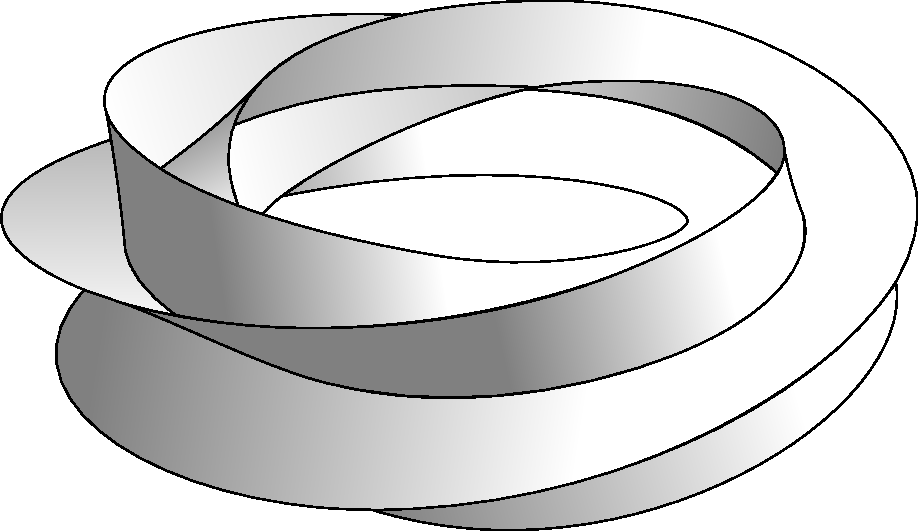
\includegraphics[width=0.7\textwidth]{img/pinwheel2.pdf}
  \caption{The "core" of the Lagrangian pinwheel $S_0 = L_{q,p}$. The pinwheel is obtained by glueing the boundary to a point.}
  \label{fig:pinwheel}
\end{figure}

To calculate the image of $B_{dpq}$ under action-angle coordinates, we can remove the segment $ℓ = [a_1^{2/p},∞] × \{0\}$ from $\im(\symbf{H})$ to obtain a simply connected domain.
Now applying the flux map gives us $τ \colon \im(\symbf{H}) ∖ ℓ → Δ$, where we define $Δ ⊂ ℝ²$ to be the image of this map, and thus giving us action-angle coordinates $μ \colon B_{dpq} ∖ \symbf{H}^{-1}(ℓ) → Δ$.
Since $\symbf{H}_2$ already generates a $S¹$ action, we may choose $τ$ to be of the form $τ(b_1,b_2) = (τ_1(b_1,b_2), b_2)$.\footnote{As when constructing action-angle coordinates in the proof of the Arnold-Liouville Theorem.}
In particular the segment $[0,a_1^{2/p}] × \{0\}$ is mapped to $[0,τ_1(a_1^{2/p},0)] × \{0\}$, even more particular $S_0$ is a Lagrangian over this segment, making it a so-called visible Lagrangian as described in \cite[Chapter 5]{evans2021atfs}.
We also know that the line $\{0\} × ℝ ⊂ \im(\symbf{H})$, consisting of elliptic-regular singularities, is sent to a straight line in some rational direction $(n,m)$.
As we have the visible Lagrangian pinwheel $S_0 = L_{p,q}$ intersecting it, by \cite[Section 5.3]{evans2021atfs}, we must have $(n,m) = (q',p)$.
After the affine linear transformation $\mqty(p & -q'\\q & p')$, with $p' = \frac{1-qq'}{p}$, the image of $τ$ is the right half plane, with the nodes sitting on a ray in direction $(p,q)$ as in \cref{fig:Bdpq_moment_image}.

Note that $μ$ can be continuously extended over all of $B_{dpq}$, even for points in $\symbf{H}^{-1}(ℓ)$.


\begin{figure}
  \centering
  \begin{tikzpicture}[scale=.7]
    \begin{scope}[shift={(-5cm,0)}]
        \fill[blue,opacity=0.2] (0,4) rectangle (8,-1);

        \draw (2,1.5) node[cross] {} (4,1.5) node[cross] {} (6,1.5) node[cross] {};
        \draw[thick] (0,4) -- (0,-1);
    \end{scope}
    \begin{scope}[shift={(5cm,0)}]
        \fill[opacity=0.1] (0,4) rectangle (8,-1);

        \draw[thick,dotted,->] (2,1) node[cross] {} -- (4,2) node[cross] {} -- (6,3) node[cross] {} -- (8,4) node[anchor=west] {$(p,q)$};
        \draw[thick] (0,4) -- (0,-1);
    \end{scope}
  \end{tikzpicture}
  \caption{Moment image of $B_{dpq}$ under $μ$}
  \label{fig:Bdpq_moment_image}
\end{figure}

\subsection{Homology of \texorpdfstring{$B_{dpq}$}{Bdpq}}
\label{sec:homology}

In order to calculate the lower bound for the displacement energy of a Lagrangian fibre torus $T(b) = μ^{-1}(\qty{b})$ for $b ∈ \im(\symbf{H})$, we will want to have calculated a basis for the homology $H_2\qty(B_{dpq},T(b))$.

$B_{dpq}$ deformation retracts to the preimage of the branch cut line segment $ℓ$ shown in red in \cref{fig:branch_cut_retraction}, by first vertically shrinking the space onto the ray $[0,∞) × \{0\}$, and then compressing the part of the ray that is to the right of all the critical points.
\todo{Das ist etwas dumm formuliert, lohnt es sich das besser zu formulieren?}

The preimage $\symbf{H}^{-1}(ℓ)$ can be understood as follows: If there were no critical points on the line, this would be a solid torus $\hat{T} = S¹×D²$ with $∂ \hat{T} = T(b)$.
We pick $(1,0),(0,1) ∈ H₁(∂ \hat{T})$ to be the classes generated by the orbits of Hamiltonian flows of $μ_1$ and $μ_2$ respectively.
For each critical fibre $k ∈ \qty{1,…,d}$ we collapse a loop along the homology class $(-q,p)$, as in \cref{fig:collapse_cycles}.
Up to homotopy this is the same as attaching a disk $D_k$ along $(-q,p)$.
Again up to homotopy we can also require that the $d$ discs $D_1,…,D_d$ are attached along $∂ \hat{T}$.
Let us call the resulting space $S$.

\begin{figure}
  \centering
  \begin{subfigure}{0.45\textwidth}
    \centering
    \begin{tikzpicture}[scale=1.8]
      \fill[blue,opacity=0.2] (0,1) rectangle (3,-1);
      \draw[thick] (0,1) -- (0,-1);
      \draw[line width=0.08cm,red,opacity=0.4,text opacity=1] (0,0) -- node[pos=0.6, anchor=north] {$ℓ$} (2.5,0);
    \fill (2.5,0)  circle[radius=1pt] node[anchor=south] {$T(b)$};
      \draw (1,0) node[cross] {} (2,0) node[cross] {};
    \end{tikzpicture}
    \caption{Retraction to branch cut line}
    \label{fig:branch_cut_retraction}
  \end{subfigure}%
  \begin{subfigure}{0.55\textwidth}
    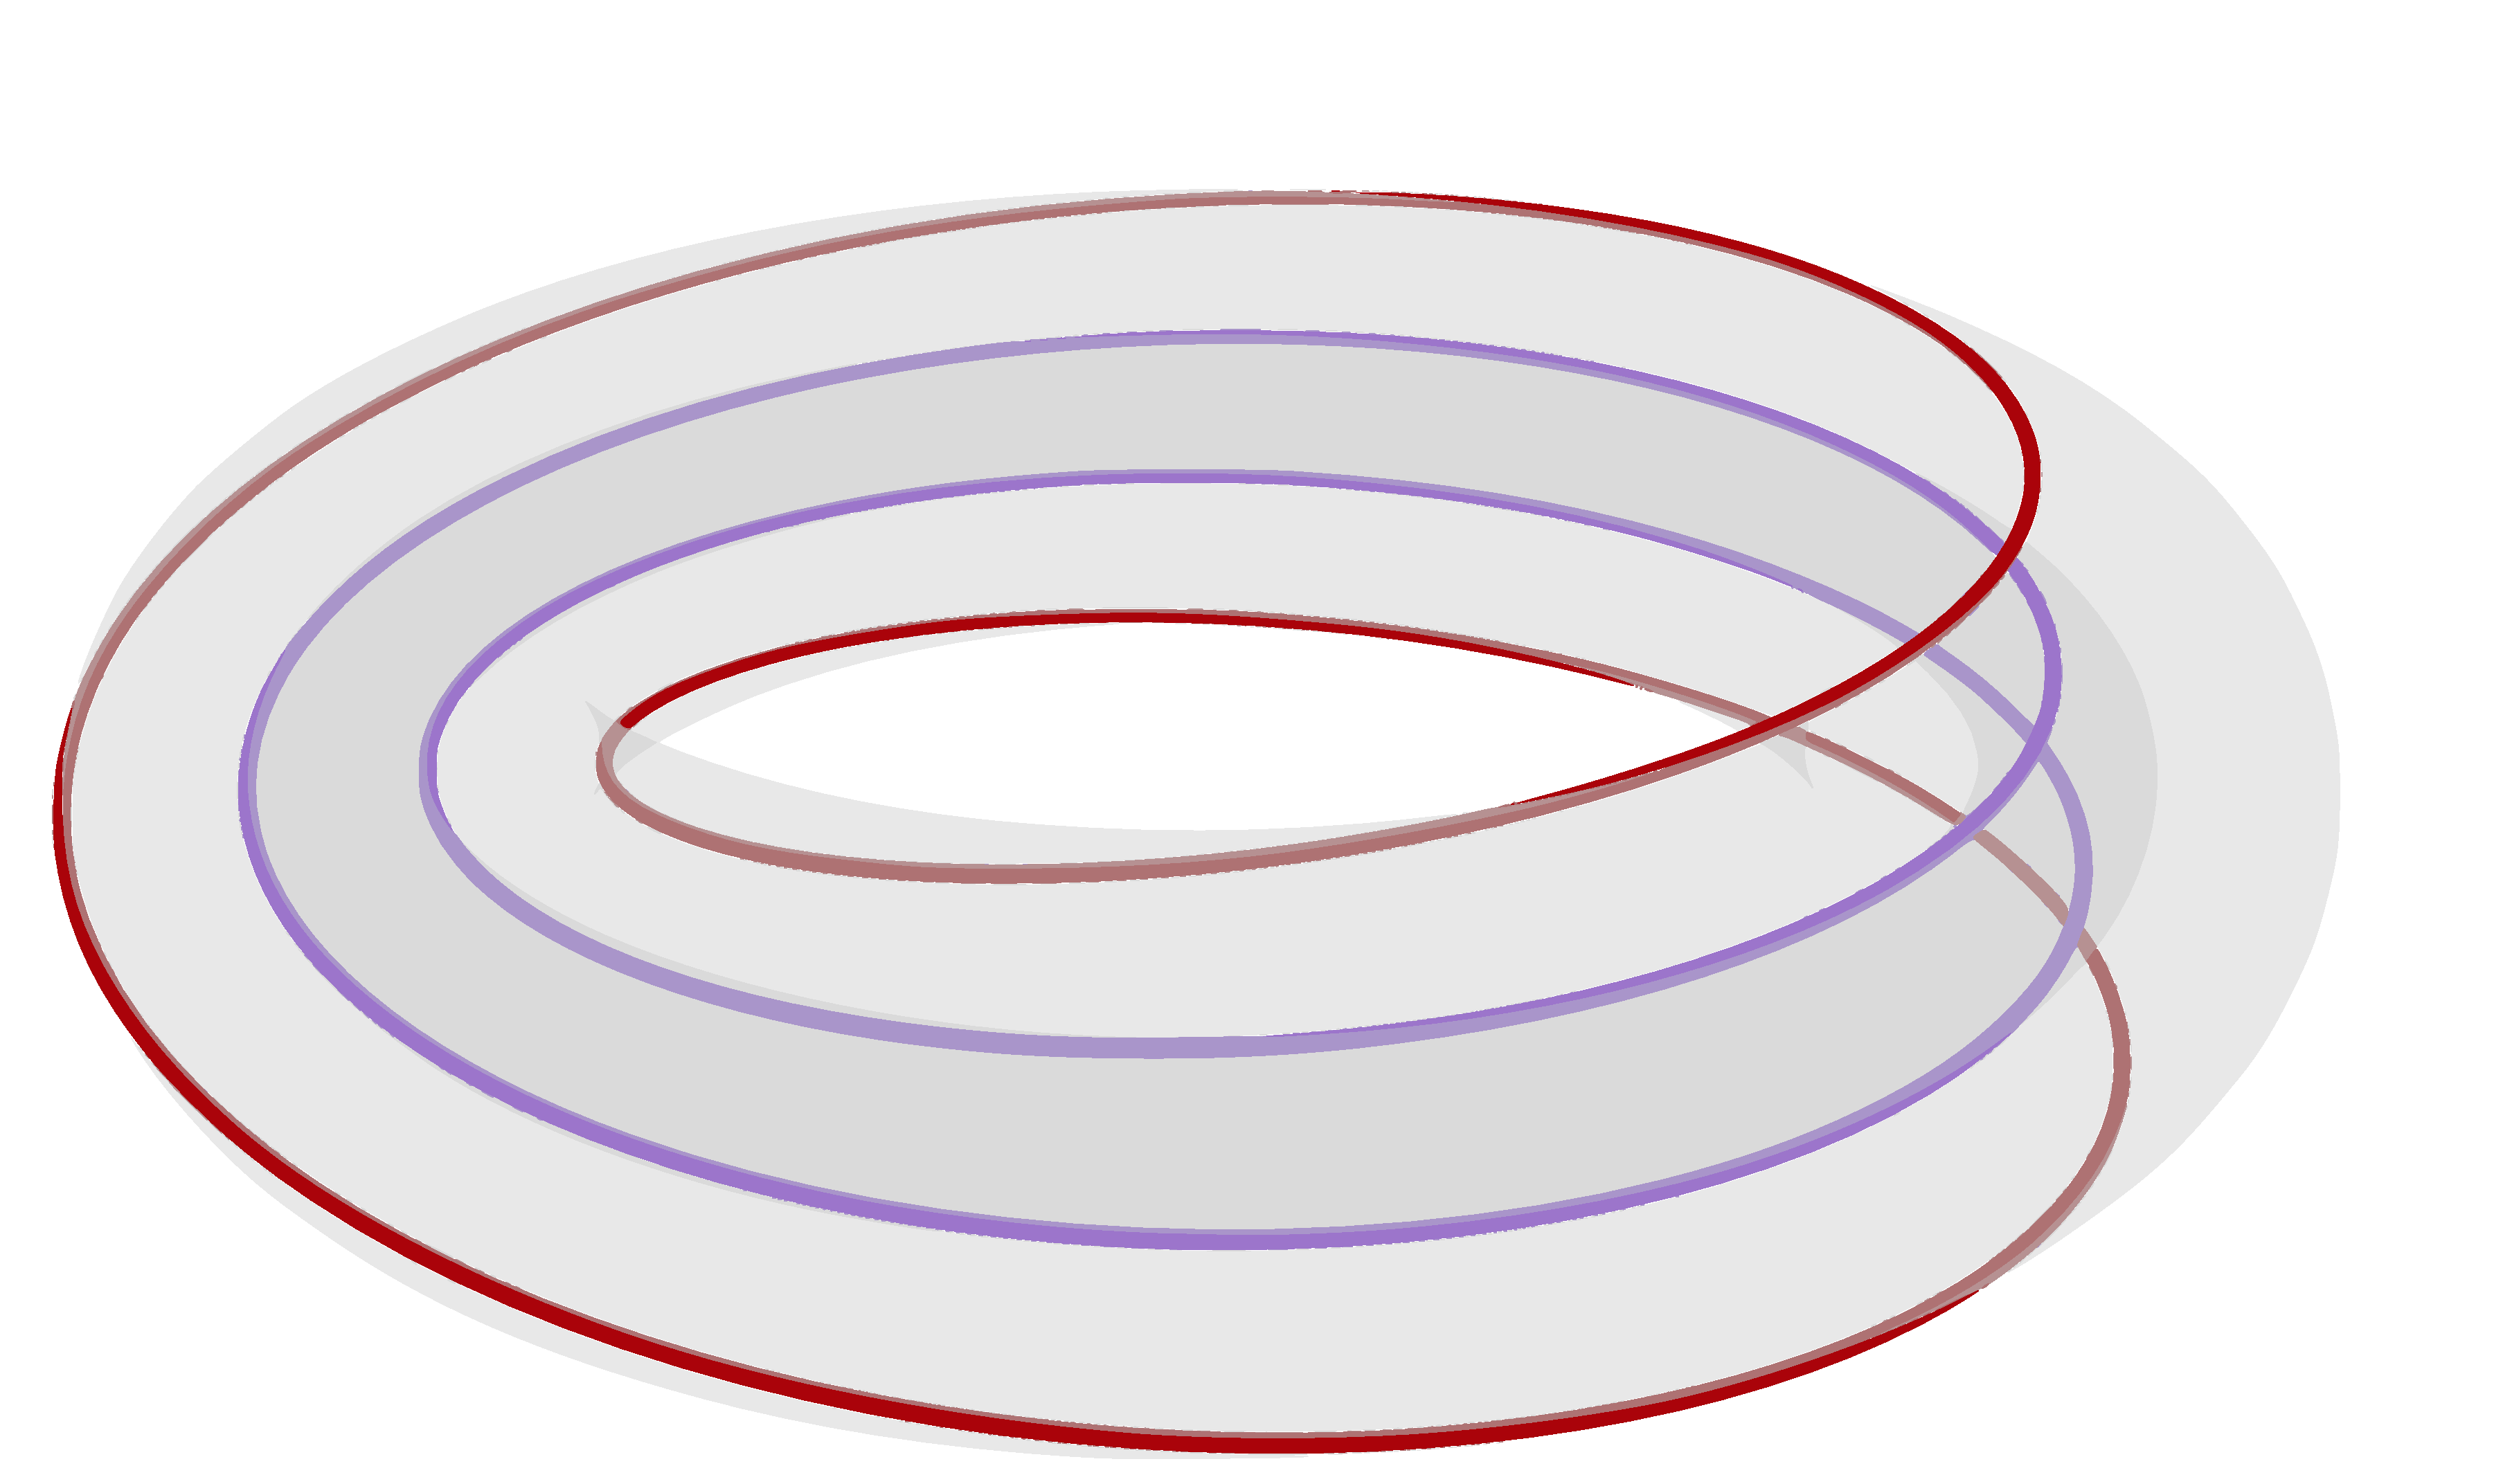
\includegraphics[width=\textwidth]{img/homology_collapse.pdf}
    \caption{The two cycles marked in red and purple (here $p=2, q=1$) are collapsed to a point.}
    \label{fig:collapse_cycles}
  \end{subfigure}
  \caption{Calculation of the homology of $B_{dpq}$}
\end{figure}

Let us look at the long exact sequence of homology for the pair $\qty(B_{dpq},T(x_1,x_2))$. This pair is homotopy equivalent to $(S,∂ \hat{T})$.

\[
\begin{tikzcd}
  H_2(∂ \hat{T}) \ar[r,"0"] &
  H_2(S) \ar[r,hook]\ar[d,"≅"] &
  H_2(S,∂ \hat{T}) \ar[r]\ar[d,"≅"] &
  H_1(∂ \hat{T}) \ar[r]\ar[d,"≅"] &
  H_1(S) \ar[d,"≅"]
  \\
  &
  ℤ^{d-1} &
  ℤ^{d+1} &
  ℤ² &
  ℤ_p
\end{tikzcd}
\]

The first horizontal map is zero since $∂ \hat{T}$ retracts to a circle in $S$.
The homology $H_2(S)$ can be seen as follows: By contracting the solid torus $\hat{T}$ in $S$ to a circle, we see that $S$ is homotopic to a circle with $d$ discs glued to its boundary by a degree $p$ map.
So $H_2(S)$ is generated by spheres $\qty{S_2,…,S_d}$, $S_k = D_{k-1}-D_{k}$.
$H_2(S,∂ \hat{T})$ is generated by the discs $D_0 = \text{pt}×D²,D₁,…,D_d$. In $B_{dpq}$, these discs can be seen, where the disc intersecting the toric boundary collapses the $(0,1)$ cycle in the toric fibre $T(x_1,x_2)$ and the discs intersecting the critical points collapse the $(-q,p)$ cycle (see \cref{fig:homology_generating_discs}).
The elements $S_2,\ldots,S_d \in H_2(B_{dpq})$ can be realized by embedded Lagragian spheres fibering over the segments between the nodes in the ATF -- these are so-called \emph{visible Lagrangians}, see \cite[Section 7.4]{evans2021atfs}.
The boundary map $∂ \colon H_2(S,∂ \hat{T}) → H_1(∂ \hat{T})$ is given by $\partial D_0 = (0,1),\, \partial D_i = (-q,p)$, meaning that the last horizontal map $H_1(∂ \hat{T}) → H_1(S)$ maps $(0,1)$ to the generator of $ℤ_p$.


\begin{figure}
  \centering
  \begin{tikzpicture}
    \fill[black!5] (0,4) rectangle (7,-1);

    \coordinate (xy) at (2.7,3.5);
    \node[anchor=south] at (xy) {$T(x_1,x_2)$};
    \fill (xy) circle[radius=.05];
    \draw (xy)
           .. controls +(0,0) and +(-.5,1) .. node[anchor=east, near end] {$D₁$} (2,1)
      (xy) .. controls +(0,0) and +(-.5,1) .. node[anchor=west, near end] {$D₂$} (4,2)
      (xy) .. controls +(0,0) and +(-.5,1) .. node[anchor=west, near end] {$D₃$} (6,3)
      (xy) .. controls +(0,0) and +(1,0) .. node[anchor=south, near end] {$D₀$} (0,2.5);

    \draw[ultra thick, blue, draw opacity=.3] (2,1) -- node[anchor=north] {$S₂$} (4,2);
    \draw[ultra thick, purple, draw opacity=.3] (4,2) -- node[anchor=north] {$S₃$} (6,3);

    \draw[thick,dotted] (2,1) node[cross] {} -- (4,2) node[cross] {} -- (6,3) node[cross] {} -- (7,3.5);

    \draw[thick] (0,4) -- (0,-1);
  \end{tikzpicture}

  \caption{The disks $D₀, …, D_d$ generating the homology $H₂\qty(B_{dpq}, T(x_1,x_2))$}
  \label{fig:homology_generating_discs}
\end{figure}

\section{Lower Bound on Displacement Energy: Minimal J-holomorphic Curves}
\label{sec:lower_bound}

We want to use the following theorem by Chekanov \cite{chekanov1998} for a lower bound of the displacement energy

\begin{theorem}
  \label{thm:chekanov}
  Let $(X,ω,J)$ be a geometrically bounded\todo{def.} symplectic manifold with $ω$-tame almost complex structure $J$\todo{Was sind die bedingungen an $J$}. Let $L ⊂ X$ be a compact Lagrangian submanifold. Then the displacement energy satisfies
  \[e(L) ≥ \min\qty{σ_D(X,L,J),σ_S(X,J)}\]
\end{theorem}
\todo{Why is $B_{dpq}$ geometrically bounded?}

To use \cref{thm:chekanov}, we can choose a suitable almost complex structure on $B_{dpq}$.

We do so in the following way: In the the construction of $B_{dpq}$ in \cref{sec:construction}, we defined $B_{dpq}$ as the quotient of $M_P$ under the free action of $ρ_p$. As a algebraic hypersurface $M_P$ naturally inherits the complex structure of $ℂ³$, and we use $J$ to denote this structure on $M_P$ as well as on its quotient $B_{dpq}$.

\begin{definition}
  Let $(M,J)$ be a almost complex manifold.
  A (smooth) function $f\colon (M,J) → ℂ$ is weakly plurisubharmonic if
  \[-\dd \dd^ℂ f = -\dd(\dd f ∘ J) ≥ 0 \;.\]
\end{definition}

The first component of $\symbf{H}$ in \ref{eqn:non-toric-system}, is a weakly plurisubharmonic function on $ℂ³$, as $-\dd \dd^ℂ \symbf{H}₁ = 2 \dd{x_3} ∧ \dd{y_3} ≥ 0$. As $M_P$ is an algebraic hypersurface, this restricts to a plurisubharmonic function on $M_P$, and also descends to the quotient $B_{dpq}$ as a plurisubharmonic function.

In particular, any $J$-holomorphic curve $u\colon Σ → B_{dpq}$ satisfies the maximum principle with respect to $\symbf{H}₁$, i.e.\ if $\symbf{H}₁ ∘ u$ has a maximum, it must be on $∂Σ$, and if $\symbf{H}₁ ∘ u$ is non-zero then it must be constant.\footnote{The latter is obtained by applying the maximum principle to $\frac{1}{\symbf{H}₁ ∘ u}$.}

\subsection{Non-Embedded lower bound}

Let $b = (b₁,b₂) ∈ \im(\symbf{H})$ and set $T = \symbf{H}^{-1}(b)$. Let $u \colon (Σ,∂Σ) → (B_{dpq},T)$ be a $J$-holomorphic curve. We have $\symbf{H}₁ ∘ u ≤ b₁$ by the maximum principle, thus $u$ is entirely contained in the region $\symbf{H}^{-1}(\qty{\symbf{H}₁ ≤ b₁})$. If we have $b₁ ≤ \symbf{H}₁(aᵢ)$, for all $1≤i≤d$, where the $a_i$ are the zeros of $P$ as in \cref{sec:homology}, then this region is homotopic to a solid torus.

Since the homology of $(\symbf{H}^{-1}(\qty{\symbf{H}_1 ≤ b_1}), T)$ is isomorphic to $ℤ$ and generated by $D₀$ as in \cref{sec:homology}, and the area of a $J$-disc rel $T$ only depends on its homology class, we have that
\[σ_D(X,T,J) ≥ ∫_{D₀} ω  = μ₁(T)\]

Since $B_{dpq}$ contains no $J$-holomorphic spheres,\footnote{As seen in \cref{sec:homology} the homology of $B_{dpq}$ is generated by Lagrangian spheres, thus any closed $J$-holomorphic curve has symplectic area $0$ and must be constant.} we have proven the following:

\begin{lemma}
  \label{thm:lower_bound_tmp}
  If $b₁ < \symbf{H}₁(aᵢ)$ for all $1 ≤ i ≤ d$, then
  \[e(B_{dpq},T) ≥ σ_D(X,T,J) ≥ ∫_{D₀} ω  = μ₁(T) \; .\]
\end{lemma}

Actually, since we are free to choose another almost complex structure, we can improve this result: 
Using a nodal slide on the moment image $μ$ as in \cref{thm:nodal_slide} we may construct a symplectomorphism $B_{P_1,q} → B_{P_2,q}$ which is a fibre-wise outside a neighbourhood of the line $\symbf{H}^{P_k,q}_2=0$, where $P_k$ are two polynomials each with $d$ distinct roots of multiplicity $p$.
For a torus $\symbf{H}^{-1}(b)$ with $b_2 ≠ 0$ we may therefore always change to a different polynomial $P_2$ where $b_1 < \symbf{H}_1(a_i)$, and choose the pullback of the natural almost complex structure of $B_{P_2,q}$. So we obtain:

\begin{lemma}
  \label{thm:lower_bound}
  If $b_2 ≠ 0$ then $e(B_{dpq},T) ≥ σ_D(X,T,J) ≥ μ₁(T)$.
\end{lemma}

\subsection{Embedded lower bound}

Let $(M,ω,J)$ be a geometrically bounded connected symplectic manifold with $ω$-tame almost complex structure $J$, denote by $g$ the associated Riemannian metric, and let $u\colon Σ → M$ be a J-holomorphic curve.

Then monotonicity (e.g. \cite[Proposition 4.3.1 (ii)]{sikorav1994}) gives us the following statement:

\begin{lemma}[Monotonicity]
  \label{thm:monotonicity}
  There exists a $C>0$ s.t.\ for all $x ∈ \im(u)$ and $B = B_r(x)$ the open ball w.r.t.\ $g$. If $u(∂Σ) ⊂ M ∖ B$ then we have
  \[∫_u ω ≥ C r²\]
\end{lemma}

As a simple corollary we get:

\begin{corollary}
  \label{cor:small_buffer}
  Suppose $∂M = ∂M^+ ⊔ ∂M^-$, with $∂M^±$ non-empty, $∂Σ = ∂Σ^+ ⊔ ∂Σ^-$, with $∂Σ^±$ non-empty and $u\colon (Σ,∂Σ) → (M,∂M)$ J-holomorphic with $u(∂Σ^±) ⊂ ∂M^±$, then
  \[∫_u ω ≥ \frac{C d(∂M^+,∂M^-)^2}{4} \; .\]
\end{corollary}

\begin{proof}
  Pick a path $γ$ from $∂Σ^-$ to $∂Σ^+$. By the intermediate value theorem there is $t$ s.t.\ $d((u ∘ γ) (t),∂M^+) = d((u ∘ γ)(t), ∂M^-)$. Picking $x = (u ∘ γ)(t)$ and using the triangle inequality we have that $B = B_{d(∂M^+,∂M^-)/2}(x) ⊂ M ∖ ∂M $. Applying \cref{thm:monotonicity} to $B$ we get the desired result.
\end{proof}

\begin{definition}
A \textbf{milnor fibre} of $B_{dpq}$ is a open subset $U$ containing $\symbf{H}^{-1}(ℓ)$, where $ℓ = [0,\symbf{H}(a_d)] × \{0\}$. \end{definition}

\begin{remark}
  This definition is a bit unusual but equivalent to the usual one.
\end{remark}

\begin{proposition}
  \label{thm:lower_bound_embedded}
  Let $φ:B_{dpq} ⊃ U → (X,ω)$ an embedding of a milnor fibre of $B_{dpq}$ into a tame symplectic manifold.

  Then there exists an $ε>0$, such that there exists a neighbourhood $V$ of $[0,ε) × \{0\} ⊂ \im{\symbf{H}}$ such that for all $b ∈ V$ with $b_2 ≠ 0$ we have $e(φ(T(b)),X) ≥ μ_1(T(b))$.
\end{proposition}

\begin{proof}
  Choose a smaller open neighbourhood $\symbf{H}^{-1}(ℓ) ⊂ U' ⊂ U$ such that $d(∂U',∂U) = s > 0$ and $U' = \symbf{H}^{-1}(V')$ for some open subset $V' ⊂ \im(\symbf{H})$ (this is possible since $\symbf{H}$ is an open map).
  Let $J$ be the natural almost complex structure on $B_{dqp}$ as in \cref{thm:lower_bound_tmp}, and $\hat{J}$ an extension of $φ_* J$ to all of $X$.


  The moment map $μ$ is given by $μ =  τ ∘ \symbf{H}$ for some diffeomorphism $τ$ defined on the complement of the branch cut line. Set $δ = \min\qty{σ_S(X,\hat{J}), \frac{Cs²}{4}}$, and set $V = V' ∩ τ^{-1}(μ_1 < δ)$.

  Let $b ∈ V$ with $b_2 ≠ 0$ and $u \colon (Σ,∂Σ) → (X,φ(T(b)))$ be a $\hat{J}$-holomorphic disk.
  If $u$ is contained in $U$, then $φ^{-1} ∘ u$ is a $J$-holomorphic disk in $B_{dpq}$ and $∫_{φ^{-1}u} ω ≥ σ_D(B_{dpq},T(b),J) ≥ e(T(b)) = μ_1(T(b)) = τ(b)$ by \cref{thm:lower_bound}.
  If not, then $u$ crosses the region $U ∖ U'$, so we can apply \cref{cor:small_buffer}, to get that $∫_u ω ≥ \frac{Cs²}{4} ≥ δ > μ_1(T(b))$.

  Since by choice of $δ$ we also have $σ_S(X,\hat{J}) ≥ μ_1(T(b))$, we can apply \cref{thm:chekanov} we get the desired result.
\end{proof}


\section{Upper bound on displacement energy: Probes}

We want to use the method of probes to calculate an upper bound on the displacement energy of certain toric fibres $T(x,y)$, i.e.\ we give a Hamiltonian diffeomorphism that displaces the $T(x,y)$ from itself.
The method to construct such a Hamiltonian diffeomorphism is the method of probes, that was first introduced by McDuff \cite{mcduff2011displacing} for exactly the same purpose.
Probes were originally introduced in the context of toric symplectic manifolds.

We quickly recall the main ideas of the method and then explain how they are applied in our situation.
Assume that $(X^{2n},\omega)$ is a toric symplectic manifold with moment map $μ \colon X → ℝ^n$ and moment polytope $\Delta$.
A \textbf{probe} $p_\lambda(w)$ is a half open line segment contained in $\Delta$, starting at a point $w \in \Delta$, where $w$ is lying on a facet of $\Delta$, pointing in the direction of $\lambda \in ℤ^n$, where the direction  $\lambda$ is integrally transverse to the facet and such that the line segment intersects the boundary of the polytope $\Delta$ only in the point $w$.
In \cite[Lemma 2.4.]{mcduff2011displacing} it is shown that if a toric fibre $\mu^{-1}(u)$ lies over a probe $p_\lambda(w)$, where $u\in \text{int}\Delta$ is strictly less than halfway along the probe, then it is displaceable.
It is worthwhile to note that this Hamiltonian displacement is local in nature.
To see this one realises that the definition probes implies that one can find an appropriate $Gl_n(\mathbb{Z})$ transformation of the $\mathbb{R^n}$ such that the facet $F$, from which the probe emanates, lies on the hyperplane $\{x_1=0\}$ and such that the direction of the probe is given by $\lambda=(1,0,\ldots,0)$.
Furthermore, there is a corresponding Darboux chart on $X$ with coordinates $z_1,\ldots,z_n$ such that the preimage under the moment map of the probe is given by
\begin{equation*}
  \mu^{-1}(p_\lambda(w))=\left\{z\in \mathbb{C}^n \mid \abs{z_1}^2<2a, \abs{z_i}=\text{const for }i\neq 1\right\},
\end{equation*}
where $a \in \mathbb{R}$ is the affine length of the probe.
By abuse of notation this information is condensed in the following diagram of symplectic reduction
\[
\begin{tikzcd}
  \left(\mu^{-1}(p_\lambda(w)),\left.\omega\right|_A\right)\ar[r,hook]\ar[d]&
  \left(\mu^{-1}(U),\left.\omega\right|_U\right)
  \\
  \left(\mathbb{D}^2(a),\omega_\text{std}\right),
\end{tikzcd}
\]
where $\mathbb{D}^2(a)\subseteq \mathbb{C}$ is the open disk enclosing area $2\pi a$.
Now a circle $S^1(b)\vcentcolon=\{z\in \mathbb{C}\mid \abs{z}^2=2b\} \subseteq \mathbb{D}^2(a)$ is displaceable by a Hamiltonian diffeomorphism of $\mathbb{D}^2(a)$ if and only if $b<\frac{a}{2}$.
The Hamiltonian generating this diffeomorphism can be extended to all of $\mathbb{C}$ in such a way that it can be lifted to $\mu^{-1}(U)$ in a compactly supported manner.

It is clear that this discussion construction extends to the case of almost toric fibrations and does trivially so, if the probe does not intersect the branch cut line.

Now assume that everything is arranged as in the assumptions and notations of \cref{thm:bdpqexotic}.
In particular the moment image associated to this setup is shown in \cref{fig:Bdpq_moment_image}.
Using the method of probes we show the upper bound on the displacement energy, i.e.


\begin{lemma}
    \label{thm:upper_bound}
  Let $U ⊂ H¹(T_k(a);ℝ) ∖ \{\text{branch cut line}\}$.
  Up to change of basis, the restriction of the displacement energy germ to $U$ is bounded from above by
  \[ \eval{\symcal{E}_{T_k(a)}}_U (x,y) \leq a+\min\{x,x(1-kpq)+ykp²\} \]
\end{lemma}

\begin{proof}
  Recall that $T_k(a)$ is the fibre over $(a,b) \in Δ_{B_{dpq}}$, where $b\vcentcolon=\frac{q}{p}a$, such that there are $k$ nodes below on the branch cut line.
  After mutating $k$ times the base point of $T_k(a)$ is contained in a neighbourhood that admits a regular torus fibration.
  The mutation process yields a new moment map $\overline{μ}$ and moment polytope $\overline{Δ_{B_{dpq}}}$
  \todo{Draw the correct picture and show the neighbourhood that is meant.} Now a neighbourhood of $0 ∈ H¹(T_k(a);ℝ)$ can be identified with a neighbourhood $V ⊂ \overline{Δ_{B_{dpq}}}$ of $(a,\frac{qa}{p}) = μ(T_k(a))$, such that $V \subset U$.
  Choose generators of $H¹(T_k(a);ℝ)$ corresponding to the components of the moment map $\overline{\mu}=(\overline{\mu_1},\overline{\mu_2})$, i.e.
  generators that are orthogonal to those.
  Using this identification a point $(x,y) ∈ H¹(T_k(a);ℝ)$ close to $0$ is sent by the versal deformation to $(a + x, b + y)$ in $\overline{Δ_{B_{dpq}}}$.
  Now the goal is to estimate the displacement energy of fibres over these points.
  This is achieved by the method of probes.
  In the moment image $\overline{Δ_{B_{dpq}}}$ horizontal probes can be used to displace all the regular toric fibres.
  Denote the Lagrangian torus fibres over $(a + x, b + y)$ by $T_{x,y}$.
  This yields 
  \[ e(B_{dpq},T_{x,y})\leq a+x. \]
  If it is above the branch cut ray,  the mutation leaves it unaffected, and the displacement energy is $x+a$.
  Note that this calculation involved a choice of basis of the cohomology vector spaces, but that the displacement energy germ is intrinsically given.\footnote{For details on displacement energy germs and versal deformations compare \cite{chekanovschlenk2015} and \cite{brendel2020real}} To compare the estimates we get for different choices of $a$'s we therefore apply the inverse mutation to get back to the original moment map $\mu$.
  The points above the branch cut are unaffected by the mutation but to the points below the branch cut line we have to apply the inverse of the anticlockwise monodromy matrix.
  \todo{Maybe include the calculations here?} A point $(a + x, b + y)$ below the branch cut line is send to $(a,b) + (x(1-kpq)+kp²y, -kq²x + y(kpq +1))$.
  Hence the displacement energy germ calculated in these coordinates is estimated by 
  \[ \eval{\symcal{E}_{T_k(a)}}_U (x,y) \leq a+\min\{x,x(1-kpq)+ykp²\}. \]
\end{proof}

\begin{theorem}
  \label{thm:upper_bound_embedded}
\end{theorem}

\section{Versal Deformations \& Nearby Lagrangians}

Fix a Lagrangian $L ⊂ (X,ω)$, and denote by $\symcal{L}$ the set of Lagrangians Lagrangian isotopic to $L$, equipped with the $\symcal{C}^1$-topology.
Denote by $\hat{\symcal{L}}$ the universal cover of $\symcal{L}$, that is the space of Lagrangian isotopies $Λ$ starting at $L$ up to endpoint preserving isotopies.

\begin{definition}
  For any Lagrangian isotopy $Λ$ starting at $L$, we have a map
  \begin{align*}
    H_1(L) &→ ℝ\\
    ξ &↦  ∫_{C_ξ} ω
  \end{align*}
  where $C_ξ$ is the cylinder obtained by sliding a representative of $ξ$ in $L$ along the Lagrangian isotopy. This is well defined (independent of the choice of $C_ξ$) and also independent by end point preserving isotopies of $Λ$.\footnote{If $C_ξ ~ C_ξ'$ by homotopy $H$, $0=∫_{∂H} ω = ∫_{C_ξ} ω - ∫_{C_ξ'} ω + ∫_A ω + ∫_B ω$, with $A,B$ contained in the endpoints of the isotopy, which are Lagrangian.}

  Using $\Hom(H_1(L),ℝ) = H^1(L;ℝ)$ this gives a well defined map
  \[\Flux \colon \hat{\symcal{L}} → H^1(L;ℝ) \; ,\]
  called the \textbf{flux map}.
\end{definition}

Suppose for a moment $X=T^* L$ with $L ⊂ T^* L$ the zero section. For any $α ∈ Ω_1(L)$, the graph $Γ_α$ of $α$ is Lagrangian iff $dα=0$. Also if $Γ_α ≅ Γ_β$ are Hamiltonian isotopic, then $α-β$ is exact. So up to Hamiltonian isotopy, Lagrangians that are graphs of one forms are classified by $H^1(L;ℝ)$ and also $\Flux(Γ_α) = [α]$.\todo{Ein paar schöne details mehr?}
Now, due to the nature of the $\symcal{C}¹$-topology on $\symcal{L}$, there is some simply connected neighbourhood $U ⊂ \symcal{L}$ of the zero section $L$, such that every $L' ∈ U$ is graph of a one form. So on this neighbourhood, $\Flux \colon U → H^1(L;ℝ)$ classifies all Lagrangians up to local Hamiltonian isotopy.

Return now to the case of a general $X$. Then $L$ admits an embedding of a Weinstein-neighbourhood $φ: T^*L \dashrightarrow X$ \footnote{The $\dashrightarrow$ notes that the map is only defined near $0$ (section)} sending the zero section onto $L$. As above, take a simply connected neighbourhood $U ⊂ \symcal{L}$ s.t.\ every $L' ∈ U$ is given as $φ(Γ_α)$ for some $α ∈ Ω_1(L)$. We call $U$ a \textbf{close neighbourhood} of $L$.

\begin{definition}
  For $U$ some close neighbourhood, a \textbf{versal deformation} of $L$ is a section of the map
  \[ \Flux\colon U → H^1(L;ℝ) \; , \]
  i.e.\ $v_L \colon H^1(L;ℝ) \dashrightarrow U$ s.t.\ $\Flux(v_L(α)) = α$.
\end{definition}

We immediately get that if $v_L,v_L'$ are two versal deformations both defined for $α ∈ H^1(L;ℝ)$, then $v_L(α) ≅ v_L'(α)$, so we might say colloquially that a versal deformations parametrizes all nearby Lagrangians by a neighbourhood of zero in $H^1(L;ℝ)$ up to local Hamiltonian isotopy.

\todo[inline]{The following are imprecice}

\begin{lemma}
  Let $\symbf{H} \colon X → ℝ^n$ be a regular Lagrangian (toric) fibration with simply connected image. Then the map $x ↦ \Flux(\symbf{H}^{-1}(\symbf{H}(x)))$ gives action angle coordinates on $X$.
\end{lemma}

\begin{lemma}
  If $μ \colon X → ℝ^n$ is a moment map with simply connected image, and $L = μ^{-1}(b_0)$, then $\Flux(μ^{-1}(b)) = b - b_0$.
\end{lemma}

\section{Proof of Main Theorem}

Combining the "non-embedded" upper and lower bounds of \cref{thm:lower_bound} and \cref{thm:upper_bound}, we immediately get:

\begin{theorem}
  \label{thm:displacement_energy}
  Let $b=(b_1,b_2) ∈ \im(\symbf{H})$ with $b_2 ≠ 0$. Then $e(\symbf{H}^{-1}(b)) = μ_1(\symbf{H}^{-1}(b)) = τ_1(b)$.
\end{theorem}

Combining the "embedded" upper and lower bounds of \cref{thm:lower_bound_embedded} and \cref{thm:upper_bound_embedded} we get:

\begin{theorem}
  \label{thm:displacement_energy_embedded}
  Let $φ \colon B_{dpq} ⊃ U → (X,ω)$ be an embedding of a milnor fibre of $B_{dpq}$ into a geometrically bounded symplectic manifold. Then there is a neighbourhood $V$ of $[0,ε) × \{0\}$ such that for $b = (b_1,b_2) ∈ V$ with $b_2 ≠ 0$ we have $e(\symbf{H}^{-1}(b)) = μ_1(\symbf{H}^{-1}(b)) = τ_1(b)$.
\end{theorem}

\begin{figure}
  \centering
  \missingfigure{$T_{kpq}$ definition}
  \caption{$T_{kpq}$}
  \label{fig:tkpq_def}
\end{figure}

\begin{definition}
  Let $0 ≤ k ≤ d$ and $a>0$.
  Using nodal slides to modify $μ$, arrange it such that the line $μ_1 = a$ separates the $k$-th and the $(k+1)$-th nodes as in \cref{fig:tkpq_def}.
  Then set $T_{k,p,q}(a) = μ^{-1}(a,\frac{aq}{p})$.
\end{definition}

\begin{theorem}
  \label{thm:main}

  For $x ∈ H^1(B_{dpq}, T_{kpq})$, the displacement energy germ at $T_{kpq}$ is given by
  \[ \symcal{E}_{T_{kpq}(a)} (x) \sim a + \min\qty{x_1, x_1 (1-kpq) + x_2 k p^2} \; . \]

If $φ \colon B_{dpq} ⊃ U → (X,ω)$ is an embedding of a Milnor fibre into a geometrically bounded symplectic manifold, and $a<ε$ as given by \cref{thm:displacement_energy_embedded}, then the same expression holds for the displacement energy germ at $φ(T_{kpq}(a))$.
\end{theorem}

\begin{figure}
  \centering
  \missingfigure{modified moment map}
  \caption{Modifiying the moment map $μ$.}
  \label{fig:mod_moment_map}
\end{figure}

\begin{proof}
  The proof of the embedded and non-embedded part are essentially the same. For simplicity we only give the non-embedded part.

  Change the branch cuts of $μ$ such that $T_{kpq}$ does not lie on a branch cut, giving a new moment map $\hat{μ}$ as in \cref{fig:mod_moment_map},
  giving the relation
  \begin{equation}
    \label{eq:mu_muhat_rel}
    \hat{μ}(z) = \begin{cases}
      μ(z) & \text{if $μ(z)$ lies above the eigenline of $A$}\\
      A μ(z) & \text{if $μ(z)$ lies below the eigenline of $A$}
    \end{cases}
  \end{equation}
  where $A$ is given as the shear matrix
  \[\mqty(kpq+1 & -kp²\\ kq² & 1-kpq) = \qty(x ↦ x+k\det\mqty(x_1 & p\\ x_2 & q)(p,q)).\]

  Choose a versal deformation $v$ at $T_{kpq}(a)$ such that
  \[
    \hat{μ}(v(x)) = \Flux(T_{kpq},v(x)) = (a,\frac{aq}{p}) + (x_1,x_2) \; .
  \]
  \todo{versal deformations schön einführen.}
  Then we know from \cref{thm:displacement_energy} (resp. \cref{thm:displacement_energy_embedded}) that for $v(x)$ not on the eigenline of the nodes, $e(v(x)) = μ_1(v(x))$.

  Applying \eqref{eq:mu_muhat_rel}, we get
  \[e(v(x)) = \begin{cases}
    μ_1(v(x)) = a + x_1 & \text{$x$ lies above the eigenline of $A$}\\
    A μ_1(v(x)) = a + x_1(kpq+1) - x_2kp² & \text{$x$ lies below the eigenline of $A$}\\
    \text{unknown} & \text{$x$ lies on the eigenline of $A$}
  \end{cases}\]

  Now we have that $kp⟨x,(q,-p)⟩ = x_1 kpq - x_2 kp^2 > 0$ iff $x$ lies above the eigenline of $A$, so we get
  \[e(v(x)) = \begin{cases}
    a + \min\qty{x_1,x_1(kpq+1) - x_2kp²} & \text{$x$ doesn't lie on the eigenline of $A$}\\
    \text{unknown} & \text{$x$ lies on the eigenline of $A$}\\
  \end{cases}\]
\end{proof}
\end{document}
